% Options for packages loaded elsewhere
\PassOptionsToPackage{unicode}{hyperref}
\PassOptionsToPackage{hyphens}{url}
\PassOptionsToPackage{dvipsnames,svgnames,x11names}{xcolor}
%
\documentclass[
  letterpaper,
  12pt,
  letterpaper]{report}

\usepackage{amsmath,amssymb}
\usepackage{setspace}
\usepackage{iftex}
\ifPDFTeX
  \usepackage[T1]{fontenc}
  \usepackage[utf8]{inputenc}
  \usepackage{textcomp} % provide euro and other symbols
\else % if luatex or xetex
  \usepackage{unicode-math}
  \defaultfontfeatures{Scale=MatchLowercase}
  \defaultfontfeatures[\rmfamily]{Ligatures=TeX,Scale=1}
\fi
\usepackage{lmodern}
\ifPDFTeX\else  
    % xetex/luatex font selection
    \setmainfont[]{Arial}
\fi
% Use upquote if available, for straight quotes in verbatim environments
\IfFileExists{upquote.sty}{\usepackage{upquote}}{}
\IfFileExists{microtype.sty}{% use microtype if available
  \usepackage[]{microtype}
  \UseMicrotypeSet[protrusion]{basicmath} % disable protrusion for tt fonts
}{}
\makeatletter
\@ifundefined{KOMAClassName}{% if non-KOMA class
  \IfFileExists{parskip.sty}{%
    \usepackage{parskip}
  }{% else
    \setlength{\parindent}{0pt}
    \setlength{\parskip}{6pt plus 2pt minus 1pt}}
}{% if KOMA class
  \KOMAoptions{parskip=half}}
\makeatother
\usepackage{xcolor}
\usepackage[top=1in,bottom=1in,left=1in,right=1in,headheight=15pt,headsep=0.3in,footskip=0.5in,includehead=false,includefoot=false]{geometry}
\setlength{\emergencystretch}{3em} % prevent overfull lines
\setcounter{secnumdepth}{-\maxdimen} % remove section numbering
% Make \paragraph and \subparagraph free-standing
\makeatletter
\ifx\paragraph\undefined\else
  \let\oldparagraph\paragraph
  \renewcommand{\paragraph}{
    \@ifstar
      \xxxParagraphStar
      \xxxParagraphNoStar
  }
  \newcommand{\xxxParagraphStar}[1]{\oldparagraph*{#1}\mbox{}}
  \newcommand{\xxxParagraphNoStar}[1]{\oldparagraph{#1}\mbox{}}
\fi
\ifx\subparagraph\undefined\else
  \let\oldsubparagraph\subparagraph
  \renewcommand{\subparagraph}{
    \@ifstar
      \xxxSubParagraphStar
      \xxxSubParagraphNoStar
  }
  \newcommand{\xxxSubParagraphStar}[1]{\oldsubparagraph*{#1}\mbox{}}
  \newcommand{\xxxSubParagraphNoStar}[1]{\oldsubparagraph{#1}\mbox{}}
\fi
\makeatother


\providecommand{\tightlist}{%
  \setlength{\itemsep}{0pt}\setlength{\parskip}{0pt}}\usepackage{longtable,booktabs,array}
\usepackage{calc} % for calculating minipage widths
% Correct order of tables after \paragraph or \subparagraph
\usepackage{etoolbox}
\makeatletter
\patchcmd\longtable{\par}{\if@noskipsec\mbox{}\fi\par}{}{}
\makeatother
% Allow footnotes in longtable head/foot
\IfFileExists{footnotehyper.sty}{\usepackage{footnotehyper}}{\usepackage{footnote}}
\makesavenoteenv{longtable}
\usepackage{graphicx}
\makeatletter
\newsavebox\pandoc@box
\newcommand*\pandocbounded[1]{% scales image to fit in text height/width
  \sbox\pandoc@box{#1}%
  \Gscale@div\@tempa{\textheight}{\dimexpr\ht\pandoc@box+\dp\pandoc@box\relax}%
  \Gscale@div\@tempb{\linewidth}{\wd\pandoc@box}%
  \ifdim\@tempb\p@<\@tempa\p@\let\@tempa\@tempb\fi% select the smaller of both
  \ifdim\@tempa\p@<\p@\scalebox{\@tempa}{\usebox\pandoc@box}%
  \else\usebox{\pandoc@box}%
  \fi%
}
% Set default figure placement to htbp
\def\fps@figure{htbp}
\makeatother
% definitions for citeproc citations
\NewDocumentCommand\citeproctext{}{}
\NewDocumentCommand\citeproc{mm}{%
  \begingroup\def\citeproctext{#2}\cite{#1}\endgroup}
\makeatletter
 % allow citations to break across lines
 \let\@cite@ofmt\@firstofone
 % avoid brackets around text for \cite:
 \def\@biblabel#1{}
 \def\@cite#1#2{{#1\if@tempswa , #2\fi}}
\makeatother
\newlength{\cslhangindent}
\setlength{\cslhangindent}{1.5em}
\newlength{\csllabelwidth}
\setlength{\csllabelwidth}{3em}
\newenvironment{CSLReferences}[2] % #1 hanging-indent, #2 entry-spacing
 {\begin{list}{}{%
  \setlength{\itemindent}{0pt}
  \setlength{\leftmargin}{0pt}
  \setlength{\parsep}{0pt}
  % turn on hanging indent if param 1 is 1
  \ifodd #1
   \setlength{\leftmargin}{\cslhangindent}
   \setlength{\itemindent}{-1\cslhangindent}
  \fi
  % set entry spacing
  \setlength{\itemsep}{#2\baselineskip}}}
 {\end{list}}
\usepackage{calc}
\newcommand{\CSLBlock}[1]{\hfill\break\parbox[t]{\linewidth}{\strut\ignorespaces#1\strut}}
\newcommand{\CSLLeftMargin}[1]{\parbox[t]{\csllabelwidth}{\strut#1\strut}}
\newcommand{\CSLRightInline}[1]{\parbox[t]{\linewidth - \csllabelwidth}{\strut#1\strut}}
\newcommand{\CSLIndent}[1]{\hspace{\cslhangindent}#1}

% ==========================================
% 1. CORE PACKAGES & UTILITIES
% ==========================================
\usepackage{booktabs}
\usepackage{longtable}
\usepackage{array}
\usepackage{multirow}
\usepackage{float}
\usepackage{graphicx}
\usepackage{tikz}
\usetikzlibrary{fadings}
\usepackage{xcolor}
\usepackage{etoolbox}
\usepackage[titles]{tocloft}
\usepackage{titlesec}
\usepackage{fancyhdr}
\usepackage{hyperref}
\usepackage[document]{ragged2e}

% --- ADD THESE LINES TO LEFT-ALIGN CAPTIONS ---
\usepackage{caption}
\captionsetup{
  justification=raggedright, % Forces left-alignment
  singlelinecheck=false      % Prevents short captions from automatically centering
}

% Type-specific overrides
\captionsetup[figure]{labelsep=period} 
\captionsetup[table]{labelsep=colon}

% --- Global Configurations ---
\graphicspath{{C:/Users/Leonardo.Durante/Documents/GitHub/ReefFish assessment/2025_Hawaii_ReefFish/}}

\hypersetup{
  colorlinks=true,
  linkcolor=black,
  urlcolor=blue,   % Keeps external web URLs blue
  citecolor=blue   % Keeps bibliographical citations blue
  linkbordercolor=blue, % Set underline border color to blue
  urlbordercolor=blue,
  citebordercolor=blue
}


% ==========================================
% 2. DOCUMENT COLORS
% ==========================================
\definecolor{noaanavy}{RGB}{0,35,100}
\definecolor{headingblue}{RGB}{0,48,135}
\definecolor{subheadingblue}{RGB}{0,133,202}
\definecolor{subsubheadingblue}{RGB}{0,141,168}
\definecolor{levelfourpurple}{RGB}{87,97,192}

% ==========================================
% 3. DOCUMENT HIERARCHY STYLES (LEVELS 1-4)
% ==========================================

% --- Part Formatting (No Label) ---
\titleclass{\part}{straight}
\titleformat{\part}[block]{\normalfont\huge\bfseries}{}{0pt}{}
\titlespacing*{\part}{0pt}{0pt}{20pt}
\makeatletter
\renewcommand{\thepart}{}
\renewcommand{\partname}{}
\makeatother

% --- Level 1: Chapter (Numbered) ---
\titleformat{\chapter}[hang]
  {\fontspec{Arial Bold}\fontsize{14pt}{16pt}\selectfont\color{headingblue}}
  {\thechapter}{1em}{}
\titlespacing*{\chapter}{0pt}{20pt}{20pt}

% --- Level 1: Chapter (Unnumbered / TOC, LOF, LOT, etc.) ---
\titleformat{name=\chapter,numberless}[hang]
  {\fontspec{Arial Bold}\fontsize{14pt}{16pt}\selectfont\color{headingblue}}
  {}{0pt}{}
\titlespacing*{name=\chapter,numberless}{0pt}{20pt}{20pt}

% --- Level 2: Section ---
\titleformat{\section}[hang]
  {\fontspec{Arial Bold}\fontsize{12pt}{14pt}\selectfont\color{subheadingblue}}
  {\thesection}{1em}{}
\titlespacing*{\section}{0pt}{20pt}{20pt}

% --- Level 3: Subsection ---
\titleformat{\subsection}[hang]
  {\fontspec{Arial Italic}\fontsize{12pt}{14pt}\selectfont\color{subsubheadingblue}}
  {\thesubsection}{1em}{}
\titlespacing*{\subsection}{0pt}{20pt}{20pt}

% --- Level 4: Subsubsection ---
\titleformat{\subsubsection}[hang]
  {\fontspec{Arial Italic}\fontsize{11pt}{13pt}\selectfont\color{levelfourpurple}}
  {\thesubsubsection}{1em}{}
\titlespacing*{\subsubsection}{0pt}{20pt}{20pt}

% ==========================================
% 4. TABLE OF CONTENTS (TOC) FORMATTING
% ==========================================

% Force normal font weights across all layout levels in TOC
\renewcommand{\cftchapfont}{\normalfont}
\renewcommand{\cftchappagefont}{\normalfont}
\renewcommand{\cftsecfont}{\normalfont}
\renewcommand{\cftsecpagefont}{\normalfont}
\renewcommand{\cftsubsecfont}{\normalfont}
\renewcommand{\cftsubsecpagefont}{\normalfont}

% Force dot leaders (........) for Main Headings, LOF, and LOT
\renewcommand{\cftchapleader}{\cftdotfill{\cftdotsep}}

% Clean internal macro patches to permanently strip Report Class bolding overrides
\makeatletter
\patchcmd{\l@chapter}{\bfseries}{\normalfont}{}{}
\patchcmd{\l@section}{\bfseries}{\normalfont}{}{}
\patchcmd{\l@subsection}{\bfseries}{\normalfont}{}{}
\makeatother

% ==========================================
% 5. LIST OF FIGURES & TABLES FORMATTING
% ==========================================
\renewcommand{\cftfigpresnum}{Figure }
\renewcommand{\cftfigaftersnum}{.}
\addtolength{\cftfignumwidth}{2.5em}

\renewcommand{\cfttabpresnum}{Table }
\renewcommand{\cfttabaftersnum}{.}
\addtolength{\cfttabnumwidth}{2.5em}

% Strip internal native header routines (Allows clean markdown control)
\makeatletter
\renewcommand{\listoffigures}{\@starttoc{lof}}
\renewcommand{\listoftables}{\@starttoc{lot}}
\makeatother

% ==========================================
% 5.1 FIX LOF/LOT TOP SPACING
% ==========================================
\makeatletter
% Patch the command that sets up the chapter header for these lists
\patchcmd{\listoffigures}{\chapter*}{\@makeschapterhead{0pt}\chapter*}{}{}
\patchcmd{\listoftables}{\chapter*}{\@makeschapterhead{0pt}\chapter*}{}{}

% Ensure the titles themselves are formatted like your other chapters
\titleformat{name=\chapter,numberless}[hang]
  {\fontspec{Arial Bold}\fontsize{14pt}{16pt}\selectfont\color{headingblue}}
  {}{0pt}{}
\titlespacing*{name=\chapter,numberless}{0pt}{-35pt}{12pt}
\makeatother

% ==========================================
% 6. RUNNING HEADERS & FOOTERS
% ==========================================
\pagestyle{fancy}
\fancyhf{}
\fancyhead{}
\renewcommand{\headrulewidth}{0pt}
\renewcommand{\footrulewidth}{0pt}

% Define the two alternating text blocks
\newcommand{\footerDOC}{\fontspec{Arial}\fontsize{11pt}{13pt}\selectfont U.S. Department of Commerce $|$ National Oceanic and Atmospheric Administration}
\newcommand{\footerNMFS}{\fontspec{Arial}\fontsize{11pt}{13pt}\selectfont National Marine Fisheries Service $|$ Pacific Islands Fisheries Science Center}

% Dynamically alternate based on even/odd page numbers
\fancyfoot[L]{\ifodd\value{page}\footerNMFS\else\footerDOC\fi}
\fancyfoot[C]{}
\fancyfoot[R]{\fontspec{Arial}\fontsize{11pt}{13pt}\selectfont \thepage}

% Mirror styles to "plain" page states (TOC/Chapter open pages)
\fancypagestyle{plain}{%
  \fancyhf{}
  \fancyfoot[L]{\ifodd\value{page}\footerNMFS\else\footerDOC\fi}
  \fancyfoot[C]{}
  \fancyfoot[R]{\fontspec{Arial}\fontsize{11pt}{13pt}\selectfont \thepage}
  \renewcommand{\headrulewidth}{0pt}
  \renewcommand{\footrulewidth}{0pt}
}

% ==========================================
% 7. APPENDIX BACKUP ROUTINE
% ==========================================
\gappto\appendix{
  \renewcommand{\appendixname}{Appendix}
  
  \titleformat{\chapter}[hang]
    {\fontspec{Arial Bold}\fontsize{14pt}{16pt}\selectfont\color{headingblue}}
    {\appendixname\ \thechapter.}{1em}{}
    
  \titleformat{name=\chapter,numberless}[hang]
    {\fontspec{Arial Bold}\fontsize{14pt}{16pt}\selectfont\color{headingblue}}
    {}{0em}{}
    
  \titlespacing*{\chapter}{0pt}{20pt}{20pt}
  \titlespacing*{name=\chapter,numberless}{0pt}{20pt}{20pt}
  
  \assignpagestyle{\chapter}{fancy}
}

%GEtting tables right
\renewcommand{\toprule}{\hline}
\renewcommand{\midrule}{\hline}
\renewcommand{\bottomrule}{\hline}
\usepackage{array}
\newcolumntype{L}[1]{>{\raggedright\arraybackslash}b{#1}}

\usepackage[nameinlink,capitalise]{cleveref}
\usepackage{booktabs}
\usepackage{longtable}
\usepackage{array}
\usepackage{multirow}
\usepackage{wrapfig}
\usepackage{float}
\usepackage{colortbl}
\usepackage{pdflscape}
\usepackage{tabu}
\usepackage{threeparttable}
\usepackage{threeparttablex}
\usepackage[normalem]{ulem}
\usepackage{makecell}
\usepackage{xcolor}
\usepackage{caption}
\usepackage{anyfontsize}
\makeatletter
\@ifpackageloaded{bookmark}{}{\usepackage{bookmark}}
\makeatother
\makeatletter
\@ifpackageloaded{caption}{}{\usepackage{caption}}
\AtBeginDocument{%
\ifdefined\contentsname
  \renewcommand*\contentsname{Table of contents}
\else
  \newcommand\contentsname{Table of contents}
\fi
\ifdefined\listfigurename
  \renewcommand*\listfigurename{List of Figures}
\else
  \newcommand\listfigurename{List of Figures}
\fi
\ifdefined\listtablename
  \renewcommand*\listtablename{List of Tables}
\else
  \newcommand\listtablename{List of Tables}
\fi
\ifdefined\figurename
  \renewcommand*\figurename{Figure}
\else
  \newcommand\figurename{Figure}
\fi
\ifdefined\tablename
  \renewcommand*\tablename{Table}
\else
  \newcommand\tablename{Table}
\fi
}
\@ifpackageloaded{float}{}{\usepackage{float}}
\floatstyle{ruled}
\@ifundefined{c@chapter}{\newfloat{codelisting}{h}{lop}}{\newfloat{codelisting}{h}{lop}[chapter]}
\floatname{codelisting}{Listing}
\newcommand*\listoflistings{\listof{codelisting}{List of Listings}}
\makeatother
\makeatletter
\makeatother
\makeatletter
\@ifpackageloaded{caption}{}{\usepackage{caption}}
\@ifpackageloaded{subcaption}{}{\usepackage{subcaption}}
\makeatother

\usepackage{bookmark}

\IfFileExists{xurl.sty}{\usepackage{xurl}}{} % add URL line breaks if available
\urlstyle{same} % disable monospaced font for URLs
\hypersetup{
  pdftitle={Opakapaka Simulation Report},
  pdfauthor={Megumi Oshima, Marc Nadon, John Syslo, Hongguang Ma, and Felipe Carvalho},
  colorlinks=true,
  linkcolor={black},
  filecolor={Maroon},
  citecolor={Blue},
  urlcolor={Blue},
  pdfcreator={LaTeX via pandoc}}


\title{Opakapaka Simulation Report}
\author{Megumi Oshima, Marc Nadon, John Syslo,Hongguang Ma, and Felipe
Carvalho}
\date{August 28, 2026}

\begin{document}
\begin{titlepage}
  \newgeometry{margin=0pt}
  
  \begin{tikzpicture}[remember picture, overlay]
  
    % Background photo cropped to the cover area without distortion
    \node[anchor=center, inner sep=0pt] at ([yshift=1in]current page.center) {%
      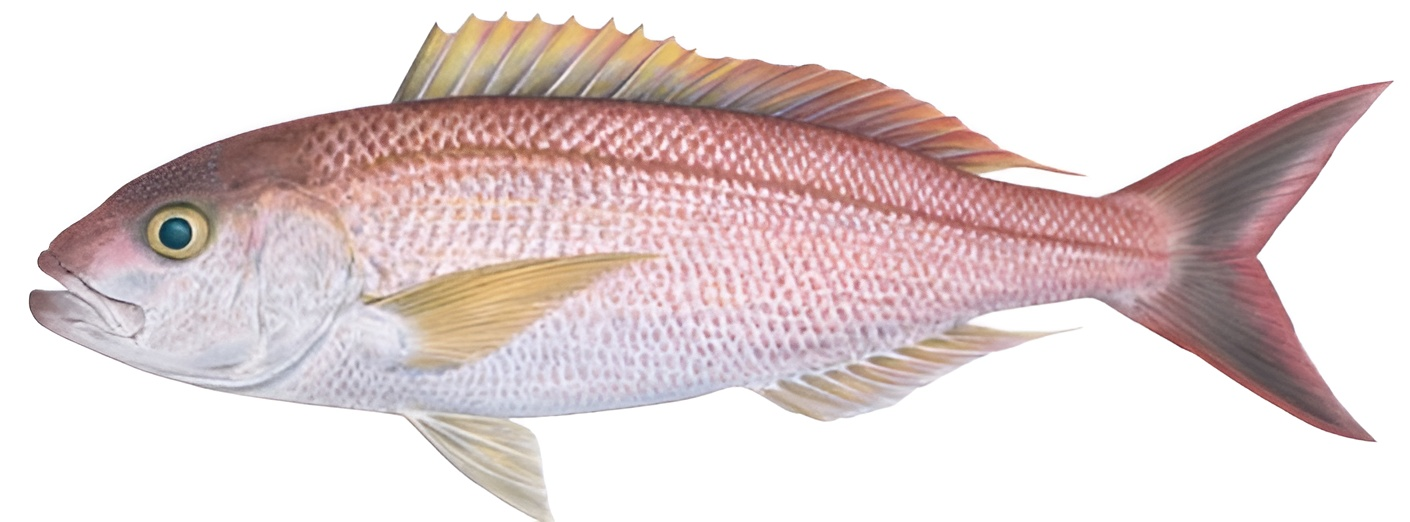
\includegraphics[width=1\paperwidth, height=0.55\paperheight, keepaspectratio, clip]{P_filamentosus.png}%
    };
    
   % NOAA logo - top left corner, full bleed
    \node[anchor=north west, inner sep=0pt] at (current page.north west) {%
      
\includegraphics[height=5.07in]{NOAA_corner_logo.png}%
    };
    
    % Navy footer bar at bottom
    \fill[noaanavy]
      (current page.south west) rectangle ++(\paperwidth, 3.5cm);
      
    % Footer text (white)
    \node[anchor=south west, text=white, inner sep=12pt, align=left,
          font=\small] at (current page.south west) {%
      NOAA Technical Memorandum NMFS-PIFSC-???\\
      U.S. Department of Commerce\\
      National Oceanic and Atmospheric Administration\\
      National Marine Fisheries Service\\
      Pacific Islands Fisheries Science Center\\
      \today
    };
    
  \end{tikzpicture}

  % Title and author text
  \vspace*{0.6\paperheight}
  \hspace{1cm}
  \begin{minipage}{0.85\textwidth}
    {\fontspec{Arial Narrow Bold}\fontsize{26pt}{30pt}\selectfont Optimizing Fishery-Independent Surveys: Evaluating Sampling Effort for the Hawaiian 'Ōpakapaka Stock Assessment \par}
    \vspace{2cm}
    {\normalsize Megumi Oshima, Marc Nadon, John Syslo, Hongguang Ma, and Felipe Carvalho\par}
  \end{minipage}
  \vfill

\end{titlepage}
\restoregeometry

% --- About/Title page ---
\clearpage
\thispagestyle{fancy}
\setcounter{page}{2}    % <--- FORCE LATEX TO LOG THIS AS PAGE 2 (Overrides cover page reset)
\vspace*{1cm}

{\fontspec{Arial Narrow Bold}\fontsize{26pt}{30pt}\selectfont Optimizing Fishery-Independent Surveys: Evaluating Sampling Effort for the Hawaiian 'Ōpakapaka Stock Assessment\par}
\vspace{1cm}

{\normalsize Megumi Oshima, Marc Nadon, John Syslo, Hongguang Ma, and Felipe Carvalho\par}
\vspace{1cm}

{\small
Pacific Islands Fisheries Science Center\\
National Marine Fisheries Service\\
1845 Wasp Boulevard\\
Honolulu, HI 96818

}



\vspace{1cm}

% Green highlight box
% Technical Memorandum Series Number Block (No Highlight)
\parbox{\textwidth}{%
  \small NOAA Technical Memorandum NMFS-PIFSC-\#\#\#\\
  {[Month]} {[Year]}
}

\vspace{1cm}


\includegraphics[width=1.3in]{900px-Seal_of_the_US_DoC.png}

\vspace{0.5cm}

{\small
U.S. Department of Commerce\\
National Oceanic and Atmospheric Administration\\
National Marine Fisheries Service\\
Pacific Islands Fisheries Science Center
}

\clearpage


%Acknowledgements
\clearpage
\thispagestyle{empty}   % <--- COMPLETELY REMOVES FOOTERS & NUMBERS FROM ACKNOWLEDGEMENTS

\vspace*{1cm}

{\fontspec{Arial Bold}\fontsize{14pt}{16pt}\selectfont Acknowledgements\par}
\vspace{0.5cm}

{\fontspec{Arial}\fontsize{12pt}{14pt}\selectfont \par}
\vspace{0.25cm}

{\fontspec{Arial}\fontsize{12pt}{14pt}\selectfont Cover drawing: Hawaiian 'Ōpakapaka \fontspec{Arial Italic}\fontsize{12pt}{14pt}\selectfont(Pristipomoides filamentosus) \fontspec{Arial}\fontsize{12pt}{14pt}\selectfont. Drawing credit: Hawai'i Division of Aquatic Resources. Artist: Les Hata.\par}
\vspace{0.25cm}

{\fontspec{Arial}\fontsize{12pt}{14pt}\selectfont Edited by --------------.\par}
\vspace{0.5cm}


{\fontspec{Arial Bold}\fontsize{14pt}{16pt}\selectfont Recommended citation\par}
\vspace{0.25cm}

{\fontspec{Arial}\fontsize{12pt}{14pt}\selectfont Oshima, M., Nadon, M., Syslo, J., Ma, H., \& Carvalho, F. (2026). Optimizing fishery-independent surveys: Evaluating sampling effort for the Hawaiian 'Ōpakapaka stock assessment (Technical Memorandum Series, TM-PIFSC-???). Pacific Islands Fisheries Science Center.\par}
\vspace{0.5cm}

{\fontspec{Arial Bold}\fontsize{14pt}{16pt}\selectfont Copies of this report are available from\par}
\vspace{0.25cm}

{\fontspec{Arial}\fontsize{12pt}{14pt}\selectfont
Pacific Islands Fisheries Science Center\\
National Marine Fisheries Service\\
National Oceanic and Atmospheric Administration\\
1845 Wasp Boulevard, Building \#176\\
Honolulu, Hawaiʻi 96818\par}
\vspace{0.5cm}


% --- Switch to Roman numerals for front matter ---
%\clearpage
%\pagenumbering{roman}

{\fontspec{Arial Bold}\fontsize{14pt}{16pt}\selectfont Or online at\par}
\vspace{0.25cm}

{\fontspec{Arial}\fontsize{12pt}{14pt}\selectfont \href{https://repository.library.noaa.gov/}{\color{blue}\underline{https://repository.library.noaa.gov/}}\par}


% --- Switch to Roman numerals for the Table of Contents page ---
\clearpage
\pagenumbering{roman}   % <--- FORCES THE TOC PAGE TO START FRESH AT ROMAN 'i'
\renewcommand*\contentsname{Table of contents}
{
\hypersetup{linkcolor=}
\setcounter{tocdepth}{1}
\tableofcontents
}

\setstretch{1.15}
\bookmarksetup{startatroot}

\chapter{List of Figures}\label{list-of-figures}

\listoffigures

\newpage{}

\bookmarksetup{startatroot}

\chapter{List of Tables}\label{list-of-tables}

\listoftables

\newpage{}

\bookmarksetup{startatroot}

\chapter*{Executive Summary}\label{executive-summary}
\addcontentsline{toc}{chapter}{Executive Summary}

\markboth{Executive Summary}{Executive Summary}

'Ōpakapaka (\emph{Pristipomoides filamentosus}) is one of Hawai'i's most
culturally significant species and is a member of the Deep 7 bottomfish
complex, a group of six deep water snapper and one grouper. The Deep 7
complex is currently assessed with a single surplus production model
however, since Crimson Jobfish comprises over 50\% of the commercial
catch of Deep 7 and is one of the few species with enough data for an
age-structured, integrated model, a single-species model has been
developed for research. One key source of information for the Deep 7
complex assessment model as well as for the Crimson Jobfish
single-species model is the Bottomfish Fishery-Independent Survey in
Hawai'i (BFISH) which provides index of abundance and length composition
data. The BFISH is an annual survey conducted around the main Hawaiian
islands since 2016 that specifically targets deep-water snapper and
grouper. The sampling design historically integrated two gear types, a
remote stereo-video camera system and a hook-and-line research fishing.
However, in response to operational and financial constraints, the
camera gear was removed from the survey and it now relies solely on
research fishing. The number of grids the BFISH surveys in a given year
has fluctuated depending on funding and logistical constraints. Because
the number of sampled grids directly impacts the uncertainty of the
abundance indices, it is important to evaluate alternative sampling
strategies to understand the relationship between number of grids
sampled and the impact on key model outputs used in management of the
fishery. We wanted to evaluate whether we could optimize the
fishery-independent survey for Crimson Jobfish by first looking at the
effect of varying levels of survey effort on the model's ability to
estimate key stock quantities under periods of normal or poor
recruitment and second, evaluate the impact of alternative gear type
(and the resulting selectivity) on the assessment model performance,
particularly under poor recruitment conditions.

We simulated 100 operating model/estimation model pairs for 14 scenarios
to test the impact of different survey efforts and gear configurations
on the Crimson Jobfish single-species model. For the poor recruitment
condition, we simulated a 40\% sustained decline in mean recruitment for
25 years. We tested five effort scenarios: high (HSE), intermediate
(ISE), low (LSE), extra low (XLSE), and none (NSE) (fishery-dependent
data only) under both normal and poor recruitment conditions. We also
tested a change in selectivity (from dome-shaped to logistic) for HSE,
ISE, and LSE efforts under poor recruitment conditions. To compare bias
and precision of each scenario, we calculated median relative error for
spawning stock biomass, fishing mortality, age-0 recruitment, and
reference points (SSB/SSB\textsubscript{MSST} and
F/F\textsubscript{MSY}).

We found that under normal recruitment conditions, all sampling
scenarios performed similarly well, with precision decreasing slightly
as effort decreased. Under poor recruitment conditions, we found that
bias increased and precision decreased as sampling effort decreased.
Additionally, the scenario with no survey effort (NSE) highlighted the
dangers of relying only on fishery-dependent data. Key management
reference points were estimated fairly well by the model at all survey
efforts but precision degraded as effort decreased. We found that under
poor recruitment, the majority of models were unable to recover the true
reference point values and that terminal year
SSB/SSB\textsubscript{MSST} was overestimated over 50\% of the time for
all effort scenarios.

We also found that changing the research fishing gear configuration from
dome-shaped to logistic had an interesting effect on model performance.
Looking at terminal year SSB specifically, for HSE and LSE, the relative
error for SSB was comparable or marginally better than the dome-shaped
selectivity model, however, for ISE, it was noticeably higher for
logistic selectivity than dome-shaped. We believe this is because of
confounding parameters and identifiability issues that are emphasized at
that level of survey effort. An informative prior on catchability under
ISE effort improved the terminal year SSB bias from 13.4\% to 7.6\%.

The results of this simulation highlight the importance of maintaining
adequate survey effort; we suggest maintaining effort levels high enough
to keep the index CV between 15-18\% for more reliable stock assessment
estimates. And particularly in times of poor recruitment, increased
monintoring should be considered. Additionally, any changes to gear
configuration may result in unexpected modelling difficulties and
adequate research should be done to understand how new gear
configurations impact catchability.

\bookmarksetup{startatroot}

\chapter{Introduction}\label{introduction}

\pagenumbering{arabic}

The Crimson Jobfish (\emph{Pristipomoides filamentosus}), locally known
as 'ōpakapaka, represents one of Hawaii's most culturally and
economically significant deep-water bottomfish species, comprising over
50\% of the total Deep-7 bottomfish catch and generating close to \$1
million annually in commercial value (Luers, DeMartini, and Humphreys
2017). As a slow-growing, long-lived species attaining up to 43 years of
age (Andrews et al. 2012) and inhabiting depths of 100-400 meters around
the Main Hawaiian Islands (Luers, DeMartini, and Humphreys 2017),
'ōpakapaka supports both vital commercial and non-commercial fisheries
that are deeply embedded in Hawaiian culture and food security. The
species is currently managed under the Western Pacific Regional Fishery
Management Council's Hawaii Fishery Ecosystem Plan as part of the Deep-7
bottomfish complex (WPRFMC 2009).

The current stock assessment model for the Deep-7 complex combines all
seven species together in a surplus production model that relies on
combined catch and index of abundance data (Syslo et al. 2024). A
single-species model for 'ōpakapaka has been developed for research and
to support the Deep-7 assessment but it has not been used for management
(Syslo et al. 2024). The dominance of 'ōpakapaka in the fishery means
that it is one of the few species out of the seven that can be assessed
with an integrated, age-structured model. One of the benefits of
transitioning to an integrated model is that it allows for the
incorporation of more data such as length or age compositions and
species-specific life-history information. However, collecting the
information that goes into an integrated assessment can be resource- and
time-intensive. Fishery-independent surveys can provide high-quality,
non-biased data that reflect the true population dynamics of targeted
species, however, they can be expensive to conduct annually. Surveys
require sufficient effort to produce quality data that informs stock
assessment models. Therefore, it is important to optimize surveys to
provide the most informative data while also balancing the costs and
time required.

The Bottomfish Fishery-Independent Survey in Hawai'i (BFISH) utilizes a
stratified-random sampling design to estimate the abundance of the
Deep-7 bottomfish complex---including 'ōpakapaka---across the main
Hawaiian Islands. Since its inception in 2016, the survey had
historically integrated two sampling modalities: remote stereo-video
camera systems and hook-and-line research fishing. However, in response
to evolving operational and financial constraints, the survey
transitioned to a single-gear approach in 2025, relying exclusively on
research fishing. Sampling is conducted within \(500 \times 500\) m
Primary Sampling Unit (PSU) grids distributed across 24 distinct strata.
A standard research fishing sample consists of 30 minutes of active
fishing within a PSU using two four-hook lines baited with squid and
fish (Richards 2025). This method provides critical species-level
identification, fork-length measurements, and life-history data.
Historically, camera deployments complemented this data, with PSU-level
metrics derived from the average of two 15-minute deployments (Richards
2025). Collectively, the camera and research fishing data are
synthesized into indices of relative abundance to inform population
trends within the Deep-7 stock assessment framework (Ducharme-Barth, N.
2023).

A well documented limitation of hook-and-line gear, however, is the
selectivity which can cause larger, older individuals to be
under-represented in catch due to gear saturation, hook size, and
avoidance behavior, producing a dome-shaped selectivity pattern relative
to the true population age/size structure ((Hommik et al. 2020;
Hutchings 2009; Garner et al. 2014)). While camera-based indices
previously offered a partial check on this limitation by sampling size
structure differently, the 2025 transition to a single-gear,
research-fishing-only design means the survey's selectivity pattern is
now determined entirely by hook-and-line gear. This raises the question
of whether modifying gear configuration to produce a more asymptotic
(logistic) selectivity pattern --- sampling proportionally more of the
older/larger portion of the population --- could improve the survey's
contribution to stock assessment, independent of any change in sampling
effort.

The scale of the BFISH survey has fluctuated over time due to logistical
and budgetary shifts. Because the total number of sampled grids directly
influences the precision of survey-derived indices, it is essential to
quantify the relationship between sampling intensity and the reliability
of stock assessment outputs. Furthermore, as environmental conditions
shift and resource constraints persist, evaluating the implications of
alternative sampling designs is necessary to optimize survey efficiency
and ensure the long-term stability of management advice.

The objective of this project was to evaluate whether we can optimize an
operational fishery-independent survey for 'ōpakapaka in the main
Hawaiian Islands. We addressed two related questions: first, the effect
of varying levels of survey effort on the ability to estimate key stock
quantities, such as spawning stock biomass, fishing mortality, and
management reference points, evaluated under two future recruitment
conditions; and second, independent of effort, whether altering research
fishing gear configuration to produce logistic rather than dome-shaped
selectivity affects assessment performance, evaluated under poor
recruitment conditions.

\bookmarksetup{startatroot}

\chapter{Methods:}\label{sec-methods}

\section{Simulation Approach}\label{simulation-approach}

We tested the impact of varying sampling efforts of a
fishery-independent survey by simulating abundance trends and data for
'ōpakapaka in the main Hawaiian islands given appropriate process and
observational error. We fit the simulated data to an age-structured
catch-at-age model and estimated spawning stock biomass, fishing
mortality, and management reference points (Syslo et al. 2024). Both the
operating model (OM) and estimation model (EM) were built in Stock
Synthesis (Methot and Wetzel 2013) (SS3) and the simulation-estimation
process was implemented using \emph{ss3sim} Johnson et al. (2024) in the
R statistical software environment (R Core Team 2024). In total, 1,400
iterations (100 iterations per scenario) were iteration using the Open
Science Grid OSG (2015). Each iteration involved (1) generating the
population dynamics from the OM, with the given F and recruitment
deviations timeseries, (2) sampling data from the OM with observational
error, and (3) fitting those data in an EM. For each iteration,
estimated quantities of interest were compared to the ``true'' values as
calculated by the OM. All code for the analysis is available in the
\href{https://github.com/noaa-pifsc/Opaka_simulation}{GitHub
repository}.

\section{Operating Model}\label{operating-model}

The operating model was a single-species, single-sex, age-structured
model conditioned on 'ōpakapaka life history parameters and historical
fishery data from the Deep-7 complex. Historical data included 75 years
of catch, CPUE, and size data from commercial and non-commercial
fisheries, plus seven years of abundance indices and length composition
data from the BFISH survey. The OM simulated population dynamics and
generated abundance indices and compositional data for 100 years.
Fishing mortality time series were generated based on historical
patterns: low values at fishery inception, increasing through the 1970s
and remaining high until the late 1990s, then declining in the early
2000s and stabilizing through the end of the time series
(Figure~\ref{fig-F-timeseries}). Annual fishing mortality values
included stochastic variability (standard deviation of 0.002) to
introduce realistic variation between iterations. Following the most
recent Deep-7 benchmark stock assessment, we applied time-varying ratios
for non-commercial catch: 1.94 from 1948-2003 and 1.09 for 2004-2049
(Syslo et al. 2024).

\begin{figure}[H]

\centering{

\pandocbounded{\includegraphics[keepaspectratio]{chapters/02_Methods_files/figure-pdf/fig-F-timeseries-1.pdf}}

}

\caption{\label{fig-F-timeseries}Fishing mortality time series for the
commercial (red lines) and non-commercial (blue lines) fisheries.}

\end{figure}%

\subsection{Recruitment Deviations}\label{recruitment-deviations}

The simulation framework was structured to evaluate estimation model
performance under varying future conditions. The first 75 years of the
100-year simulation represented the historical period with known data
patterns, while the final 25 years constituted ``future years'' designed
to test the robustness of the estimation model against potential changes
in recruitment dynamics. Two distinct recruitment scenarios were
implemented for these future years to bracket plausible recruitment
conditions: (1) a ``normal'' recruitment scenario that maintained
historical mean recruitment levels with no systematic change over time,
and (2) a ``poor recruitment'' scenario that imposed a 40\% decline in
mean recruitment relative to historical levels. This approach allowed us
to assess whether survey sampling intensity affects the estimation
model's ability to detect and respond to recruitment shifts that could
significantly impact stock productivity and sustainable harvest levels.
A total of 200 recruitment deviation time series were generated, 100
were independent, bias-corrected lognormal random deviates with a
standard deviation (\(σ_R\)) of 0.52 for the entire 100 years, and the
remaining 100 were the same for the first 75 years and then the last 25
years were calculated to drive a decline in recruitment.

The baseline recruitment level was established using the mean
recruitment from the most recent 15-year period (280,000 individuals),
representing contemporary recruitment conditions prior to the simulated
decline.

The declining recruitment scenario was structured as a two-phase process
spanning 25 years. Phase 1 comprised a 10-year transition period
characterized by a smooth exponential decline from baseline recruitment.
The annual porportional rate of change (\emph{r}) was calculated as: \[
r = (M_{target}^(\frac{1}{10})) - 1
\] where \(M_{\text{target}}\) represents the recruitment multiplier at
year 10 relative to baseline. Because recruitment remains above the
reduced state during the 10-year transition phase and varies
non-linearly with spawning biomass, \(M_{\text{target}}\) was
iteratively solved to achieve an overall 40\% reduction in long-term
mean expected recruitment (60\% of baseline). This yielded
\(M_{\text{target}} = 0.62\), corresponding to an annual decline rate of
\(r\approx-4.67\%\). Phase 2 maintained recruitment at
\(M_{\text{target}} = 0.62\) for the remaining 15 years, simulating a
persistent regime shift to lower productivity.

Annual recruitment multipliers (\(M_t\)) across both phases were
calculated as:

\[
M_t = \begin{cases} (1 + r)^t, & 1 \le t \le 10 \\ M_{\text{target}}, & 11 \le t \le 25 \end{cases}
\]

Projected deterministic recruitment values (\(R_t = \bar{R} \cdot M_t\))
were converted to recruitment deviations in log-space to maintain
consistency with stock assessment model parameterization: \[
\delta_t = \ln\left(\frac{R_t}{\bar{R}}\right)
\] where \(\bar{R}\) is the baseline mean recruitment (279.67). No
bias-correction term was applied at this step because \(\delta_t\) is a
deterministic quantity, not a random draw, so there is no lognormal
inflation to correct for.

To incorporate realistic recruitment variability around the
deterministic decline trend, we generated 100 Monte Carlo iterations of
the low-recruitment time series. For each iteration \(i\), final
recruitment deviations (\(\delta_{t,i}\)) were calculated by adding
random process noise (\(\varepsilon_{t,i}\)), bias-corrected so that the
stochastic realizations were centered on the deterministic trend: \[
\delta_{t,i} = \delta_t + \varepsilon_{t,i} - \frac{\sigma^2}{2}, \quad \text{where } \varepsilon_{t,i} \sim N(0, 0.15^2)
\]

This additional stochastic noise (\(\sigma = 0.15\)) was intentionally
set smaller than the baseline recruitment variability
(\(\sigma_R = 0.52\)) to ensure the underlying decline signal remained
statistically detectable above the noise.

\begin{figure}[H]

\centering{

\pandocbounded{\includegraphics[keepaspectratio]{chapters/02_Methods_files/figure-pdf/fig-rec_dev-1.pdf}}

}

\caption{\label{fig-rec_dev}Log recruitment deviations for one iteration
used in the normal (red solid line) and poor (blue dashed line)
recruitment scenarios.}

\end{figure}%

\subsection{Initial Fishing Mortality and
Selectivity}\label{initial-fishing-mortality-and-selectivity}

Initial instantaneous fishing mortality was fixed at 0.012 for the
commercial fishery and assumed to start at equilibrium for the
non-commercial fishery. Logistic selectivity was modeled for the
commercial and non-commercial fisheries and a dome-shaped double normal
selectivity model was used for the research fishing survey
(Figure~\ref{fig-selex}).

\begin{figure}[H]

\centering{

\pandocbounded{\includegraphics[keepaspectratio]{chapters/02_Methods_files/figure-pdf/fig-selex-1.pdf}}

}

\caption{\label{fig-selex}Selectivity functions used for the commercial
(blue line), non-commercial (orange line), and survey (red line).}

\end{figure}%

\subsection{Observation Error
Specification}\label{observation-error-specification}

Sampling error (variability in data sampled from the OM) and observation
error specified in the EM were the same, ensuring no misspecification of
uncertainty. The CV and effective sample size parameters remained
constant across all years within each scenario (Table~\ref{tbl-sas}).

\section{Scenarios}\label{scenarios}

We evaluated five sampling scenarios to assess how different levels of
survey effort affect stock assessment performance under each recruitment
condition (Table~\ref{tbl-sas}). Survey effort was defined by the number
of sampling grids covered, which directly influenced the precision of
the resulting abundance index and length composition data. Catch, CPUE,
and length composition data were simulated from the OM based on the
population dynamics generated by the specific F and recruitment
deviation time series (Figure~\ref{fig-data}).

\subsection{Survey Effort Scenarios}\label{survey-effort-scenarios}

The scenarios ranged from high survey effort (HSE) with 632 grids to
extra low survey effort (XLSE) with only 257 grids. As expected, higher
effort translated to more precise data: index CVs ranged from 15\% (HSE)
to 30\% (XLSE), and effective sample sizes for length compositions
ranged from 60 (HSE) to 15 (XLSE). The no survey effort scenario (NSE)
represented a baseline case where stock assessments would rely solely on
fishery-dependent data.

\begin{table}

\caption{\label{tbl-sas}The observational error used to sample data from
the OM for high survey effort (HSE), intermediate survey effort (ISE),
low survey effort (LSE), extra low survey effort (XLSE), and no survey
effort (NSE) for effort-based scenarios and selectivity-based scenarios.
For each survey effort, the number of sampling grids (Grids) that effort
would translate to, the resulting index of abundance CV, and effective
sample size for length composition data are shown. All effort-based
scenarios were tested under both normal and poor recruitment conditions,
while selectivity-based scenarios were tested only under poor
recruitment conditions.}

\centering{

\fontsize{12.0pt}{14.4pt}\selectfont
\begin{tabular*}{\linewidth}{@{\extracolsep{\fill}}lcrrr}
\toprule
{\bfseries Type} & Scenario & Grids & CV & effN \\ 
\midrule\addlinespace[2.5pt]
Effort & NSE & 0 & 0.20 & 0 \\ 
Effort & XLSE & 257 & 0.30 & 15 \\ 
Effort & LSE & 407 & 0.24 & 30 \\ 
Effort & ISE & 557 & 0.18 & 45 \\ 
Effort & HSE & 632 & 0.15 & 60 \\ 
Selectivity & LSE-Selectivity & 407 & 0.24 & 30 \\ 
Selectivity & ISE-Selectivity & 557 & 0.18 & 45 \\ 
Selectivity & ISE-Selectivity-q-prior & 557 & 0.18 & 45 \\ 
Selectivity & HSE-Selectivity & 632 & 0.15 & 60 \\ 
\bottomrule
\end{tabular*}

}

\end{table}%

\subsection{Selectivity Scenarios}\label{selectivity-scenarios}

Independent of survey effort, we evaluated whether the shape of survey
selectivity affects assessment performance. We simulated an alternative
gear configuration, producing a logistic selectivity and applied it
under poor recruitment conditions at three of the survey effort levels,
HSE, ISE, and LSE (Table~\ref{tbl-sas}). CV and effective sample sizes
for the selectivity scenarios were the same as their counterparts with
dome-shaped selectivity (e.g.~HSE-selectivity CV = HSE CV)
(Table~\ref{tbl-sas}). XLSE was not included in the selectivity
comparison because this effort level represents a worst case scenario in
terms of survey effort and not a likely case.

\subsection{Catchability Prior Sensitivity
Analysis}\label{catchability-prior-sensitivity-analysis}

Preliminary results indicated that logistic selectivity introduces
confounding between estimated survey catchability (\(q\)) and SSB at
intermediate effort. To test whether this identifiability issue could be
resolved with modest external information, we re-ran the ISE-selectivity
poor recruitment scenario with an informative lognormal prior on
\(ln(q)\), centered on the OM value with SD = 0.1.

\subsection{Hyperstability in Fishery
Data}\label{hyperstability-in-fishery-data}

For the NSE scenario under poor recruitment conditions, we incorporated
hyperstability into the commercial CPUE data to reflect realistic
fishery behavior during population decline (NSE-hyperstable). The CPUE
and catch data were modified to not fully reflect the underlying
population decline, simulating the tendency of commercial fisheries to
maintain catch rates even as fish abundance decreases through improved
fishing efficiency, targeting behavior, or fishing in higher-density
areas.

\subsection{Data Sources by Scenario}\label{data-sources-by-scenario}

All scenarios had some combination of catch, abundance index, and length
composition data available for the EM (Figure~\ref{fig-data}). For all
survey scenarios (HSE through XLSE), commercial CPUE and length data
were discontinued after 2023, forcing the estimation model to rely
entirely on survey-based abundance and length data for the final 25
years. This design allowed us to isolate the effect of survey data
quality on assessment performance. In contrast, the NSE scenarios
continued using commercial fishery data throughout the entire time
series.

\begin{figure}[H]

\centering{

\pandocbounded{\includegraphics[keepaspectratio]{chapters/02_Methods_files/figure-pdf/fig-data-1.pdf}}

}

\caption{\label{fig-data}Data generated from operating models and used
in the estimation models with the survey (a) and the estimation models
without the survey (b). The size of each point represents the relative
amount of data available per year and fleet (i.e.~large points represent
years with more data).}

\end{figure}%

\section{Estimation Model}\label{estimation-model}

The only structural difference in the EM from the OM was that for the
poor recruitment condition, a recruitment regime time block was
introduced for the last 15 years. Without the regime, the model was
unable to fit the persistant decline in recruitment and the relative
errors in outputs were over exaggerated. When fitting the model, all
parameters were fixed except for \(R_0\), the regime parameter for the
poor recruitment scenarios, catchability for the commercial and survey
fleets, and selectivity parameters for the commercial fishery and survey
fleet.

\section{Performance Indices}\label{performance-indices}

To compare the bias and precision of each sampling strategy, we compared
the relative error (RE) between the OM and EM for spawning stock biomass
(SSB), fishing mortality (F), age-0 recruitment, and reference points
SSB/SSB\textsubscript{MSST} and F/F\textsubscript{MSY}. Bias was
described by the median relative error (MRE)

\[
MRE = median(\frac{EM - OM}{OM})
\]

where EM is the estimated value from the EM and OM is the true value
from the OM, and precision was described by the variability in relative
error across iterations. In particular, we report the bias and precision
in the terminal year as this provides information on the long-term
impacts of sampling effort on assessment and management abilities. We
also evaluated the probability that the terminal year reference points
(SSB/SSB\textsubscript{MSST} and F/F\textsubscript{MSY}) were 10\%
greater or smaller than the true reference point values. We believe that
managers should be cautious of estimates that fall outside of 10\% of
the true value.

\bookmarksetup{startatroot}

\chapter{Results}\label{results}

Out of 1,400 EM runs, 65 runs did not converge (maximum gradient was
greater than 1e-4). The models with logistic selectivity under poor
recruitment conditions had the lowest convergence rates, ranging from
82-85\% convergence. Out of the scenarios with dome-shaped selectivity,
the NSE scenarios were the only ones that had iterations that did not
converge. Overall, model convergence for all sampling scenarios was
high.

\section{Normal Recruitment
Conditions}\label{normal-recruitment-conditions}

Under normal recruitment, all sampling strategies exhibited similar bias
and precision for terminal-year SSB (Table~\ref{tbl-re-term-yr}).
Relative error remained low, ranging from 2\% (\(SD = 0.154\)) to 3.6\%
(\(SD = 0.136\)). Notably, the NSE scenario---relying solely on
commercial CPUE and length data---performed nearly as well as the
highest-effort scenarios. This high performance in the NSE scenario
likely stems from the small CV associated with the fishery CPUE index
that the survey replaces and robust effective sample sizes for fishery
length data. For scenarios with surveys, precision for SSB over the
final 25 years scaled with sampling intensity (Figure~\ref{fig-mre}).
For instance, the 95\% error interval of SSB for the XLSE scenario was
wider (--22\% to 38\%) than that of the HSE (--12\% to 28\%), which
could have significant influence on reference point estimation.

\begin{table}

\caption{\label{tbl-re-term-yr}Median relative error and standard
deviation of relative error in the terminal year for spawning biomass,
recruitment, and fishing mortality by scenario.}

\centering{

\fontsize{12.0pt}{14.4pt}\selectfont
\begin{tabular*}{\linewidth}{@{\extracolsep{\fill}}crrr}
\toprule
Scenario & {\bfseries Spawning Biomass} & {\bfseries Fishing Mortality} & {\bfseries Recruitment} \\ 
\midrule\addlinespace[2.5pt]
\multicolumn{4}{l}{{\bfseries Normal Recruitment}} \\[2.5pt] 
\midrule\addlinespace[2.5pt]
NSE & 0.036 (0.100) & -0.031 (0.100) & 0.359 (0.931) \\ 
XLSE & 0.020 (0.154) & -0.024 (0.151) & 0.304 (1.400) \\ 
LSE & 0.036 (0.136) & -0.029 (0.130) & 0.351 (1.410) \\ 
ISE & 0.026 (0.115) & -0.025 (0.110) & 0.350 (1.412) \\ 
HSE & 0.035 (0.109) & -0.033 (0.103) & 0.353 (1.418) \\ 
\midrule\addlinespace[2.5pt]
\multicolumn{4}{l}{{\bfseries Poor Recruitment}} \\[2.5pt] 
\midrule\addlinespace[2.5pt]
NSE & 0.386 (0.294) & 0.012 (0.206) & 0.533 (0.404) \\ 
XLSE & 0.144 (0.192) & -0.122 (0.162) & 0.150 (0.267) \\ 
LSE & 0.133 (0.169) & -0.120 (0.139) & 0.209 (0.264) \\ 
LSE-Selectivity & 0.150 (0.168) & -0.134 (0.142) & 0.212 (0.261) \\ 
ISE & 0.129 (0.146) & -0.117 (0.124) & 0.237 (0.254) \\ 
ISE-Selectivity & 0.146 (0.148) & -0.128 (0.124) & 0.223 (0.258) \\ 
HSE & 0.128 (0.133) & -0.111 (0.113) & 0.212 (0.238) \\ 
HSE-Selectivity & 0.119 (0.136) & -0.109 (0.116) & 0.224 (0.244) \\ 
\bottomrule
\end{tabular*}

}

\end{table}%

\begin{figure}[H]

\centering{

\pandocbounded{\includegraphics[keepaspectratio]{chapters/03_Results_files/figure-pdf/fig-mre-1.pdf}}

}

\caption{\label{fig-mre}Timeseries of median (solid line) and 95\%
quantile (band) relative error of spawing stock biomass for the high
(HSE), intermediate (ISE), low (LSE), extra low (XLSE), and no survey
effort (NSE) scenarios under both the normal and poor recruitment
conditions.}

\end{figure}%

Fishing mortality exhibited similar bias and precision across all
scenarios in the terminal year, though estimates were consistently lower
than true values (Table~\ref{tbl-re-term-yr}). Terminal-year \(F\) MRE
ranged from --2.4\% (\(SD = 0.151\)) to --3.3\% (\(SD = 0.103\)).
Notably, while the XLSE scenario showed a slightly lower bias, it also
demonstrated the lowest precision. Conversely, the HSE
scenario---despite having slightly higher bias---offered superior
precision. The marginal 1\% increase in bias in the HSE is a negligible
trade-off for the gain in precision and may simply be a simulation
artifact. Consistent with SSB patterns precision for \(F\) over the
final 25 years declined as sampling effort decreased for scenarios with
surveys (Figure~\ref{fig-Fmre}). The 95\% error interval for the XLSE
scenario {[}--23\%, 31\%{]} was wider than the more constrained
{[}--18\%, 18\%{]} range of the HSE.

\begin{figure}[H]

\centering{

\pandocbounded{\includegraphics[keepaspectratio]{chapters/03_Results_files/figure-pdf/fig-Fmre-1.pdf}}

}

\caption{\label{fig-Fmre}Timeseries of median (solid line) and 95\%
interval (band) relative error of fishing mortality for the high (HSE),
intermediate (ISE), low (LSE), extra low (XLSE), and no survey effort
(NSE) scenarios under both the normal and poor recruitment conditions.}

\end{figure}%

Over the final 25-year period, the HSE and ISE scenarios provided the
most accurate estimates of true age-0 recruitment, while the XLSE
scenario performed the poorest---particularly in the most recent years
(Figure~\ref{fig-recmre}). Although the XLSE recorded the lowest MRE in
the terminal year (Table~\ref{tbl-re-term-yr}), terminal-year
recruitment estimates are inherently unreliable due to limited data
observations. A persistent overestimation of age-0 recruitment across
all models likely explains the positive bias observed in SSB during the
final years of the simulation. Generally, the variability in RE for
recruitment was substantially higher than for SSB or \(F\)
(Table~\ref{tbl-re-term-yr}), indicating that the estimation model
struggles to precisely capture recruitment dynamics regardless of
sampling effort.

\begin{figure}[H]

\centering{

\pandocbounded{\includegraphics[keepaspectratio]{chapters/03_Results_files/figure-pdf/fig-recmre-1.pdf}}

}

\caption{\label{fig-recmre}Timeseries of median (solid line) and 95\%
interval (band) relative error of age-0 recruitment for the high (HSE),
intermediate (ISE), low (LSE), extra low (XLSE), and no survey effort
(NSE) scenarios under both the normal and poor recruitment conditions.}

\end{figure}%

Under normal recruitment, all models showed similar bias when estimating
stock status (\(SSB/SSB_{MSST}\) and \(F/F_{MSY}\)), but precision
degraded noticeably as sampling effort decreased
(Figure~\ref{fig-refpoints}). The NSE scenario had precision levels
comparable to the HSE, given the low CV associated with the fishery CPUE
index. Median relative error for \(SSB/SSB_{MSST}\) ranged from 2.3\% to
4\% across scenarios (Table~\ref{tbl-refpoints}), with precision
(standard deviation) varying from 0.100 (NSE) to 0.153 (XLSE). The 4\%
precision gap between the XLSE and HSE scenarios represents a meaningful
difference that could influence management decisions. Similarly, the MRE
for \(F/F_{MSY}\) was tightly clustered between 2.8\% and 3.1\% for all
scenarios (Table~\ref{tbl-refpoints}). However, the standard deviation
again revealed a 0.04 discrepancy between the HSE and XLSE. This
suggests that while all sampling intensities yield similar point
estimates for terminal-year \(F/F_{MSY}\), reduced effort compromises
precision and increases the risk of significant under- or
overestimation.

Lastly, the reliability of key reference point estimates remained
consistent across all scenarios under normal recruitment conditions
(Table~\ref{tbl-prob-wrong}). The likelihood of incorrectly estimating
\(SSB/SSB_{MSST}\) (defined as a deviation \(>10\%\)) was under 50\% for
nearly all scenarios, ranging from 51\% in the LSE to 30\% in the NSE.
Similarly, the probability of an incorrect \(F/F_{MSY}\) estimate was
below 50\% for all scenarios, reaching a minimum of 29\% in the NSE.
These results indicate that under normal recruitment, current sampling
efforts generally produce estimates within a 10\% margin of the true
value the majority of the time.

\begin{figure}[H]

\centering{

\pandocbounded{\includegraphics[keepaspectratio]{chapters/03_Results_files/figure-pdf/fig-refpoints-1.pdf}}

}

\caption{\label{fig-refpoints}Distirbution of relative error for
terminal year SSB, spawning stock biomass at minimum stock size
threshold (SSB\_MSST), the terminal year stock status (SSB/SSB\_MSST),
terminal year F, FMSY, and terminal year fishing status (F/FMSY).}

\end{figure}%

\begin{table}

\caption{\label{tbl-refpoints}Median relative error and standard
deviation of relative error in the terminal year for
SSB/SSB\textsubscript{MSST} and F/F\textsubscript{MSY} by scenario.}

\centering{

\fontsize{12.0pt}{14.4pt}\selectfont
\begin{tabular*}{\linewidth}{@{\extracolsep{\fill}}crr}
\toprule
Scenario & SSB/SSB\textsubscript{MSST} & F/F\textsubscript{MSY} \\ 
\midrule\addlinespace[2.5pt]
\multicolumn{3}{l}{{\bfseries Normal Recruitment}} \\[2.5pt] 
\midrule\addlinespace[2.5pt]
NSE & 0.035 (0.100) & -0.028 (0.101) \\ 
XLSE & 0.023 (0.153) & -0.028 (0.152) \\ 
LSE & 0.028 (0.136) & -0.029 (0.132) \\ 
ISE & 0.031 (0.115) & -0.030 (0.111) \\ 
HSE & 0.040 (0.109) & -0.031 (0.105) \\ 
\midrule\addlinespace[2.5pt]
\multicolumn{3}{l}{{\bfseries Poor Recruitment}} \\[2.5pt] 
\midrule\addlinespace[2.5pt]
NSE & 0.389 (0.293) & 0.013 (0.205) \\ 
XLSE & 0.149 (0.191) & -0.117 (0.161) \\ 
LSE & 0.145 (0.168) & -0.124 (0.140) \\ 
LSE-Selectivity & 0.162 (0.164) & -0.134 (0.137) \\ 
ISE & 0.140 (0.145) & -0.117 (0.122) \\ 
ISE-Selectivity & 0.148 (0.147) & -0.122 (0.124) \\ 
HSE & 0.128 (0.132) & -0.115 (0.112) \\ 
HSE-Selectivity & 0.127 (0.134) & -0.106 (0.113) \\ 
\bottomrule
\end{tabular*}

}

\end{table}%

\begin{table}

\caption{\label{tbl-prob-wrong}Probability that reference points
SSB/SSB\textsubscript{MSST} and F/F\textsubscript{MSY} are above or
below 10\% from the true value for each scenario.}

\centering{

\fontsize{12.0pt}{14.4pt}\selectfont
\begin{tabular*}{\linewidth}{@{\extracolsep{\fill}}crr}
\toprule
Scenario & SSB/SSB\textsubscript{MSST} & F/F\textsubscript{MSY} \\ 
\midrule\addlinespace[2.5pt]
\multicolumn{3}{l}{{\bfseries Normal Recruitment}} \\[2.5pt] 
\midrule\addlinespace[2.5pt]
NSE & 0.30 & 0.29 \\ 
XLSE & 0.49 & 0.49 \\ 
LSE & 0.51 & 0.44 \\ 
ISE & 0.43 & 0.44 \\ 
HSE & 0.39 & 0.37 \\ 
\midrule\addlinespace[2.5pt]
\multicolumn{3}{l}{{\bfseries Poor Recruitment}} \\[2.5pt] 
\midrule\addlinespace[2.5pt]
NSE & 0.85 & 0.58 \\ 
XLSE & 0.67 & 0.67 \\ 
LSE & 0.68 & 0.64 \\ 
LSE-Selectivity & 0.66 & 0.65 \\ 
ISE & 0.68 & 0.62 \\ 
ISE-Selectivity & 0.65 & 0.65 \\ 
HSE & 0.65 & 0.60 \\ 
HSE-Selectivity & 0.65 & 0.57 \\ 
\bottomrule
\end{tabular*}

}

\end{table}%

\section{Poor Recruitment Conditions}\label{poor-recruitment-conditions}

Under poor recruitment conditions, most sampling scenarios exhibited
comparable bias and precision for SSB (Figure~\ref{fig-mre}) and \(F\)
(Figure~\ref{fig-Fmre}). However, overall model performance degraded
significantly compared to normal recruitment conditions. The
NSE-hyperstable scenario was an expected outlier, performing
substantially worse than all other configurations with an SSB
terminal-year MRE of 38.6\% (\(SD = 0.294\))
(Table~\ref{tbl-re-term-yr}). For all other scenarios, SSB MRE was more
moderate, ranging from 11.9\% (\(SD = 0.136\)) in HSE to 14.4\%
(\(SD = 0.192\)) in XLSE.

Similarly, estimates of \(F\) were less accurate under poor recruitment
(Figure~\ref{fig-Fmre}). MRE for \(F\) ranged from 1.2\%
(\(SD = 0.206\)) in NSE-hyperstable to --12.2\% (\(SD = 0.162\)) in the
XLSE (Table~\ref{tbl-re-term-yr}). Interestingly, while the
NSE-hyperstable scenario yielded the lowest bias for \(F\) over the
final decade, it was characterized by much higher variability throughout
the projection period (\(SD = 0.206\)), making the estimates less
reliable for consistent management.

Age-0 recruitment was estimated with similar accuracy in all scenarios
except the NSE-hyperstable (Figure~\ref{fig-recmre}).
Counter-intuitively, terminal-year recruitment estimates were less
biased under poor recruitment than under normal recruitment conditions
(Table~\ref{tbl-re-term-yr}). Furthermore, precision was notably higher
across all scenarios---including the NSE-hyperstable---throughout the
entire projection period (Figure~\ref{fig-recmre}).

The HSE scenario demonstrated the strongest performance for estimating
terminal-year \(SSB/SSB_{MSST}\) and \(F/F_{MSY}\)
(Figure~\ref{fig-refpoints}). This scenario produced the lowest
variability, with MREs of 12.8\% for \(SSB/SSB_{MSST}\) and --11.5\% for
\(F/F_{MSY}\) (Table~\ref{tbl-refpoints}). Conversely, the NSE scenario
performed the poorest for \(SSB/SSB_{MSST}\), with an MRE of 38.9\%
(\(SD = 0.293\)). Critically, the true terminal-year stock status was
not recovered in the majority of simulation runs for any scenario, as
interquartile ranges failed to include zero. This suggests that under
poor recruitment, all tested models tend to provide an overly optimistic
view of stock status. The only exception was \(F/F_{MSY}\) under the
NSE-hyperstable scenario, where the MRE was near zero; however, this
accuracy comes with a trade-off of extreme uncertainty. The wide range
of relative error in the NSE-hyperstable scenario increases the risk of
severe overestimation of \(F/F_{MSY}\), potentially leading to
unnecessary fishery closures or drastic allocation reductions.

The probability of significant estimation error (deviating \(>10\%\)
from the true value) is markedly higher under poor recruitment
conditions (Table~\ref{tbl-prob-wrong}). The likelihood of incorrectly
estimating \(SSB/SSB_{MSST}\) exceeded 50\% for all sampling scenarios,
reaching 85\% in the NSE. Similarly, the probability of an incorrect
\(F/F_{MSY}\) estimate was greater than 50\% for all scenarios, reaching
67\% for the XLSE scenario.

\subsection{Effect of Survey
Selectivity}\label{effect-of-survey-selectivity}

Independent of survey effort, changing the research survey gear to
produce logistic rather than dome-shaped selectivity affected SSB
estimation, but the effect was not uniform across effort levels
(Figure~\ref{fig-selectivity-comparison}). At HSE, logistic selectivity
performed comparably to --- or marginally better than --- dome
selectivity (SSB MRE 11.0\% vs.~11.9\%), (Table~\ref{tbl-re-term-yr}).
At ISE, logistic selectivity produced noticably higher bias than dome
(SSB MRE of 13.4\% vs.~12.1\%) (Table~\ref{tbl-re-term-yr}). And at LSE,
the two converged again (13.6\% vs.~13.3\%). This pattern suggests the
impact of selectivity shape is concentrated at intermediate survey
effort, where there is enough information for the estimation model to
converge confidently on a biased solution, but not enough to resolve it.

This effort-dependent pattern was traced to the confounding of survey
catchability and SSB: across all scenarios, terminal-year SSB relative
error was strongly correlated with \(q\) relative error (r = 0.71--0.89)
(Figure~\ref{fig-q-ssb-cor}), consistent with the known identifiability
issue between \(q\) and an asymptotic selectivity curve that lacks an
interior peak to anchor scale. Applying an informative prior on
\(\ln(q)\) in the ISE logistic-selectivity scenario reduced SSB MRE from
13.4\% to 7.6\% and substantially tightened the distribution (SD went
from 0.148 to 0.104), supporting catchability identifiability as the
mechanism driving the degraded performance under logistic selectivity at
intermediate effort.

\begin{figure}[H]

\centering{

\pandocbounded{\includegraphics[keepaspectratio]{chapters/03_Results_files/figure-pdf/fig-selectivity-comparison-1.pdf}}

}

\caption{\label{fig-selectivity-comparison}Median relative error of
terminal year spawning stock biomass for the high (HSE), intermediate
(ISE), and low (LSE) scenarios with dome-shaped (red bars), logistic
selectivity (blue bars), and logistic selectivity with an informative
prior on q (green bar).}

\end{figure}%

\begin{figure}[H]

\centering{

\pandocbounded{\includegraphics[keepaspectratio]{chapters/03_Results_files/figure-pdf/fig-q-ssb-cor-1.pdf}}

}

\caption{\label{fig-q-ssb-cor}Probability that reference points
SSB/SSB\textsubscript{MSST} and F/F\textsubscript{MSY} are above or
below 10\% from the true value for each scenario.}

\end{figure}%

\bookmarksetup{startatroot}

\chapter{Discussion}\label{discussion}

Our results show that the value of a fishery-independent survey is not
fixed, it depends on the stability of recruitment, the reliability of
the fishery-dependent index, and as our selectivity scenarios
demonstrated, on survey design choices such as gear configuration that
interact with sampling effort in ways that are not always intuative.
Under normal recruitment, sampling effort primarily dictates the
precision rather than the accuracy of biomass and fishing mortality
estimates. However, this relationship shifts fundamentally under poor
recruitment conditions or regime-type shifts. In these scenarios, survey
effort becomes a determinant of both precision and the ability to
accurately characterize stock status. Additionally, a change in gear
configuration may not automatically improve the accuracy of estimates, a
miminum amount of information is needed for the model to be able to
identify and estimate scaling parameters well.

The poor recruitment scenarios revealed a significant optimism bias
across all models. When recruitment declined, the interquartile ranges
for \(SSB/SSB_{MSST}\) and \(F/F_{MSY}\) consistently failed to capture
the true values, providing an overly favorable view of stock status.
This bias was exacerbated by reduced sampling effort. High and
intermediate survey effort scenarios (HSE and ISE) demonstrated
comparable performance across all metrics, including median relative
error and standard deviation of relative error. Lower effort scenarios
(LSE and XLSE) maintained similar central tendency measures but
exhibited substantially wider confidence intervals, indicating reduced
precision in parameter estimates. This pattern illustrates how poor
recruitment conditions amplify the negative consequences of reduced
sampling effort, creating a compounding effect where assessment
reliability deteriorates precisely when accurate population monitoring
becomes most critical for management decisions. The performance
degradation observed below intermediate effort levels suggests that
survey coverage should target a CV between 15-18\% for 'ōpakapaka stock
management, either through an optimization of the sampling design or
maintaining a sufficient number of grids. This is particularly the case
given the potential for unexpected recruitment variability in this
system.

The NSE scenarios exemplify why it is dangerous to rely soley on
fishery-dependent CPUE indices to track population trends. The fishery
index provided a complete timeseries of informative data that allowed
the model to accurately estimation population size. However, this was
only true under the normal recruitment conditions and once a decline in
recruitment was introduced, the model performed far worse than the
others in almost every metric. A major assumption of the NSE model is
that the fishery data, particularly the CPUE and size data are
accurately characterizing the full population. This is likely untrue, as
fishers are knowledgeable about where and when to find larger fish and
will likely be able to maintain a healthy catch even if the population
is declining (i.e.~hyperstability). Therefore, we should not assume that
fishery-dependent data is an accurate, unbiased representation of the
true population dynamics.

A key finding of this study is that the effect of gear selectivity on
assessment performance was not uniform across sampling effort levels,
but instead concentrated at intermediate effort
(Table~\ref{tbl-re-term-yr}, Figure~\ref{fig-selectivity-comparison}).
Switching from dome-shaped to logistic selectivity produced negligble
change in SSB relative error at HSE and LSE, but increased median
relative error from 12.9\% to 14.6\% at ISE. This pattern is consistent
with a known identifiability issues between catchability and selectivity
in age-structured stock assessment models ((Maunder and Piner (2015))).
HSE likely provided enough independent information to resolve the
confounding despite it, while at LSE the confounding was outweighed by
the substantially larger observation error already present in the
composition and index data. ISE represents an intermediate condition:
sufficient information for the model to converge confidently on a
solution, but insufficient to resolve the catchability-selectivity
confound, resulting in a consistent, well-defined bias rather than added
noise. This was further supported by a targeted sensitivity analysis in
which applying an informative prior on catchability reduced median SSB
relative error at ISE from 13.4\% to 7.6\%, directly implicating
catchability identifiability, rather than selectivity shape per se, as
the underlying mechanism.

These results suggest that the consequences of gear-selectivity changes
for a fishery-independent survey cannot be evaluated independently of
the survey's overall sampling effort, and that intermediate-precision
surveys --- a common target for cost-constrained monitoring programs ---
may be particularly susceptible to this form of bias. For BFISH
specifically, this implies that any gear modification intended to
improve sampling of larger, older 'ōpakapaka should be evaluated jointly
with expected survey precision, and that a catchability prior informed
by independent data (e.g., a gear calibration or paired-tow study) may
be a more practical mitigation than attempting to resolve the confound
through effort alone. We note that this pattern was identified across
only three effort levels and a single recruitment scenario; testing
additional effort levels and confirming the interaction under normal
recruitment conditions would strengthen confidence that this represents
a general property of logistic-selectivity surveys rather than a feature
specific to the scenarios tested here.

Our simulation relied on several key assumptions that may not fully
capture the complexity of real-world fishery dynamics and data
collection challenges. The NSE-hyperstable scenario under poor
recruitment assumed complete hyperstability in fishery data, meaning
catch rates remained unaffected by population decline throughout the
25-year projection period. While hyperstability is a documented
phenomenon in fishery-dependent CPUE indices, sustained recruitment
failure would eventually manifest in commercial catch data, suggesting
our model may have overestimated the NSE-hyperstable scenario's
limitations. Nevertheless, this represents a plausible ``worst-case''
scenario that highlights the risks of relying solely on
fishery-dependent data during periods of stock decline. Additionally,
our model simplified future data availability by excluding fishery CPUE
and length composition data after 2023, which artificially increased
uncertainty even in high survey effort scenarios. In practice, these
fishery data streams would continue but would be appropriately weighted
within the assessment framework to balance their influence against
survey observations. Finally, the poor recruitment scenarios employed
reduced variability in recruitment deviations to clearly establish
declining trends, whereas natural recruitment variability typically
remains high even during periods of decline. This simplification may
have amplified the apparent impacts of recruitment failure, as realistic
variability could obscure declining trends and complicate early
detection of regime shifts.

While consistent long-term monitoring remains ideal, a combination of
adaptive sampling strategies and improved data collection techniques
could help balance assessment reliability with resource constraints. An
adaptive approach could involve reducing survey effort during periods
when recruitment appears stable and population indicators show no signs
of decline, then increasing sampling intensity when early warning
signals suggest recruitment failure or population stress. However, such
adaptive strategies must be implemented cautiously, as maintaining data
continuity over extended periods provides irreplaceable value for
detecting long-term trends and regime shifts. Complementary improvements
to data collection could enhance assessment quality without necessarily
increasing survey effort, such as incorporating annual age data from the
fishery-independent survey to better understand population structure and
recruitment dynamics, or refining research fishing methodology in the
BFISH survey to reduce coefficient of variation in indices of abundance.

These results highlight several critical considerations for fishery
management. The first is that maintaining adequate survey effort is
essential for reliable stock assessments, particularly for fishing
mortality estimates used in management decisions. The second is that
during periods of recruitment failure, enhanced rather than reduced
monitoring may be necessary to maintain assessment reliability. We saw a
noticeable decrease in our estimation abilities when recruitment was
poor and there was a reduced survey effort. Additionally, scientists and
managers should account for increased uncertainty in stock status during
periods of both poor recruitment and reduced survey effort (even under
normal recruitment conditions). Lastly, changes in gear type may cause
additional difficulties in the model if there is not enough information
in the data (i.e.~effort is not high enough).

\bookmarksetup{startatroot}

\chapter*{Literature Cited}\label{literature-cited}
\addcontentsline{toc}{chapter}{Literature Cited}

\markboth{Literature Cited}{Literature Cited}

\phantomsection\label{refs}
\begin{CSLReferences}{1}{0}
\bibitem[\citeproctext]{ref-ss3sim2014}
Anderson, Sean C., Cole C. Monnahan, Kelli F. Johnson, Kotaro Ono, and
Juan L. Valero. 2014. {``Ss3sim: An {R} Package for Fisheries Stock
Assessment Simulation with {Stock Synthesis}.''} \emph{PLOS ONE} 9 (4):
e92725. \url{https://doi.org/10.1371/journal.pone.0092725}.

\bibitem[\citeproctext]{ref-andrews_long-lived_2012}
Andrews, Allen H., Edward E. DeMartini, Jon Brodziak, Ryan S. Nichols,
and Robert L. Humphreys. 2012. {``A Long-Lived Life History for a
Tropical, Deepwater Snapper ({Pristipomoides} Filamentosus): Bomb
Radiocarbon and Lead--Radium Dating as Extensions of Daily Increment
Analyses in Otoliths.''} \emph{Canadian Journal of Fisheries and Aquatic
Sciences} 69 (11): 1850--69. \url{https://doi.org/10.1139/f2012-109}.

\bibitem[\citeproctext]{ref-ducharme-barth_n_model-based_2023}
Ducharme-Barth, N. 2023. {``Model-Based Relative Abundance Indices for
the Main {Hawaiian} {Islands} {Deep} 7 Bottomfish Complex, 2016-2022.''}

\bibitem[\citeproctext]{ref-garner_experimental_2014}
Garner, Steven B., III Patterson William F., Clay E. Porch, and Joseph
H. Tarnecki. 2014. {``Experimental {Assessment} of {Circle} {Hook}
{Performance} and {Selectivity} in the {Northern} {Gulf} of {Mexico}
{Recreational} {Reef} {Fish} {Fishery}.''} \emph{Marine and Coastal
Fisheries} 6 (1): 235--46.
\url{https://doi.org/10.1080/19425120.2014.952463}.

\bibitem[\citeproctext]{ref-Hommik-2020}
Hommik, Kristiina, Colm J. Fitzgerald, Fiona Kelly, and Samuel Shephard.
2020. {``Dome-Shaped Selectivity in LB-SPR: Length-Based Assessment of
Data-Limited Inland Fish Stocks Sampled with Gillnets.''}
\emph{Fisheries Research} 229: 105574.
https://doi.org/\url{https://doi.org/10.1016/j.fishres.2020.105574}.

\bibitem[\citeproctext]{ref-Hutchings-2009}
Hutchings, Jeffrey A. 2009. {``Avoidance of Fisheries-Induced Evolution:
Management Implications for Catch Selectivity and Limit Reference
Points.''} \emph{Evolutionary Applications} 2 (3): 324--34.
https://doi.org/\url{https://doi.org/10.1111/j.1752-4571.2009.00085.x}.

\bibitem[\citeproctext]{ref-R-ss3sim}
Johnson, Kelli F., Sean C. Anderson, Kathryn L. Doering, Cole C.
Monnahan, and Christine C. Stawitz. 2024. \emph{Ss3sim: Fisheries Stock
Assessment Simulation Testing with Stock Synthesis}.
\url{https://github.com/ss3sim/ss3sim}.

\bibitem[\citeproctext]{ref-luers_seasonality_2017}
Luers, Meagan A., Edward E. DeMartini, and Robert L. Humphreys. 2017.
{``Seasonality, Sex Ratio, Spawning Frequency and Sexual Maturity of the
Opakapaka {Pristipomoides} Filamentosus ({Perciformes}: {Lutjanidae})
from the {Main} {Hawaiian} {Islands}: Fundamental Input to
Size-at-Retention Regulations.''} \emph{Marine and Freshwater Research}
69 (2): 325--35. \url{https://doi.org/10.1071/MF17195}.

\bibitem[\citeproctext]{ref-maunder-piner-2015}
Maunder, Mark N., and Kevin R. Piner. 2015. {``Contemporary Fisheries
Stock Assessment: Many Issues Still Remain.''} \emph{ICES Journal of
Marine Science} 72 (1): 7--18.
\url{https://doi.org/10.1093/icesjms/fsu015}.

\bibitem[\citeproctext]{ref-methot_stock_2013}
Methot, Richard D., and Chantell R. Wetzel. 2013. {``Stock Synthesis:
{A} Biological and Statistical Framework for Fish Stock Assessment and
Fishery Management.''} \emph{Fisheries Research} 142 (May): 86--99.
\url{https://doi.org/10.1016/J.FISHRES.2012.10.012}.

\bibitem[\citeproctext]{ref-https:ux2fux2fdoi.orgux2f10.21231ux2f906p-4d78}
OSG. 2006. {``OSPool.''} OSG. \url{https://doi.org/10.21231/906P-4D78}.

\bibitem[\citeproctext]{ref-https:ux2fux2fdoi.orgux2f10.21231ux2f0kvz-ve57}
---------. 2015. {``Open Science Data Federation.''} OSG.
\url{https://doi.org/10.21231/0KVZ-VE57}.

\bibitem[\citeproctext]{ref-osg07}
Pordes, Ruth, Don Petravick, Bill Kramer, Doug Olson, Miron Livny, Alain
Roy, Paul Avery, et al. 2007. {``The Open Science Grid.''} In \emph{J.
Phys. Conf. Ser.}, 78:012057. 78th Series.
\url{https://doi.org/10.1088/1742-6596/78/1/012057}.

\bibitem[\citeproctext]{ref-R-core-team}
R Core Team. 2024. \emph{R: A Language and Environment for Statistical
Computing}. Vienna, Austria: R Foundation for Statistical Computing.
\url{https://www.R-project.org/}.

\bibitem[\citeproctext]{ref-richards_annual_2025}
Richards, Benjamin. 2025. {``Annual {Report}: 2024 {Bottomfish}
{Fishery}-{Independent} {Survey} in {Hawaiʻi}.''} \emph{NOAA Technical
Memorandum NMFS PIFSC ; 177}. \url{https://doi.org/10.25923/059V-F791}.

\bibitem[\citeproctext]{ref-osg09}
Sfiligoi, Igor, Daniel C Bradley, Burt Holzman, Parag Mhashilkar, Sanjay
Padhi, and Frank Wurthwein. 2009. {``The Pilot Way to Grid Resources
Using glideinWMS.''} In \emph{2009 WRI World Congress on Computer
Science and Information Engineering}, 2:428--32. 2nd Series.
\url{https://doi.org/10.1109/CSIE.2009.950}.

\bibitem[\citeproctext]{ref-syslo_benchmark_2024}
Syslo, John, Megumi Oshima, Hongguang Ma, Nicholas Ducharme-Barth, Marc
Nadon, and Felipe Carvalho. 2024. {``Benchmark Stock Assessment for the
Main {Hawaiian} {Islands} {Deep} 7 Bottomfish Complex, with Projections
Through 2029.''} \url{https://doi.org/10.25923/5SSG-8D54}.

\bibitem[\citeproctext]{ref-wprfmc_fishery_2009}
WPRFMC. 2009. {``Fishery {Ecosystem} {Plan} for the {Hawaii}
{Archipelago}.''} Western Pacific Regional Fishery Management Council.
\url{http://www.wpcouncil.org/fishery-plans-policiesreports/hawaii-fishery-ecosystem-plan}.

\end{CSLReferences}




\end{document}
